\documentclass[conference]{IEEEtran}
\IEEEoverridecommandlockouts
% The preceding line is only needed to identify funding in the first footnote. If that is unneeded, please comment it out.
\usepackage{cite}
\usepackage{amsmath,amssymb,amsfonts}
\usepackage{algorithmic}
\usepackage{graphicx}
\usepackage{textcomp}
\usepackage{xcolor}
\usepackage{tabularx}
\usepackage{hyperref}

\usepackage{fancyhdr}
\pagestyle{fancy}
\lhead{Michigan Robotic Submarine}
\rhead{\thepage}

\def\BibTeX{{\rm B\kern-.05em{\sc i\kern-.025em b}\kern-.08em
    T\kern-.1667em\lower.7ex\hbox{E}\kern-.125emX}}

\newcolumntype{L}{>{\raggedright\arraybackslash}X} % This column type allows the text in the table with "Component Specifications" to be left aligned (as opposed to full justification)

\begin{document}

\title{Michigan Robotic Submarine: Strategy, Design, and Implementation of Theseus}
\author{
Arnav Mummineni, Melissa Peters, Luke VanderHeuvel % Team leads
\\ 
Muskaan Mittal, Kaden Chirco, Nathan Kuo, Carter Kassin, Zayn Baig, Ashley McPike % Other members
}


\maketitle
\pagestyle{fancy}
\lhead{Michigan Robotic Submarine}
\rhead{\thepage}

\begin{abstract}
Michigan Robotic Submarine is an undergraduate student project team at the University of Michigan in its fourth year participating in the RoboSub competition. We developed our autonomous underwater vehicle (AUV), Theseus, shown in Fig. 1, to improve our accuracy and reliability on previous tasks, opening potential for future developments. To improve iteration speed, we developed a new bottom plate with additional component mounting points. To simplify our electrical system, we redesigned and consolidated our flight controller and motor control systems, removing redundant components. We continued to develop our task planning framework to decrease error potential and increase reliability. Finally, we laid the groundwork for future improvement like improved localization and control using our DVL, additional mechanisms to complete new tasks, and adding electrical safety mechanisms to prevent future damage and setbacks.

\end{abstract}

\section{Competition Strategy} \label{sec:comp_strat}
This year we focused on increasing reliability on the tasks we attempted previously and adapting to the modified tasks, such as the change from the buoy to the slalom. Our recent changes to our system demonstrate its strong modularity and its ability to improve over time to tackle this year’s and future years’ RoboSub challenges. Some areas that we identified as strengths included our machine learning pipeline, which we were able to quickly train and utilize at previous competitions along with a robust task planner to map out the failure cases and fallback states for each task. In turn, we continued to develop our classical computer vision pipeline and design additional mechanisms.

\subsection{Target Tasks} \label{ssec:target_goals}
Our target tasks for the 2025 RoboSub competition are the coin flip, gate, slalom, and bin tasks.
\begin{enumerate}
\item \textit{Heading Out---Coin Flip:}
To complete the coin flip task, our design requires the robot to be sensing its environment before starting the run so that it can record the angle that the gate is present at. This provides a reliable method for identifying the initial angle needed to turn to face the gate, regardless of the result of the coin flip. 
\item \textit{Collecting Data---Gate:}
To pass through the gate, we use a machine learning model to detect the image on the gate and center on it. We decided to always choose the same image to center on, as this allows us to focus on optimizing the model’s performance for that specific image. Additionally, this makes it so that we can complete the bin and slalom tasks in the same way every run to maximize points (namely, the same side of the slalom poles and the same side to target on the bin), enabling more consistency throughout our runs.

\begin{figure}
    \centerline{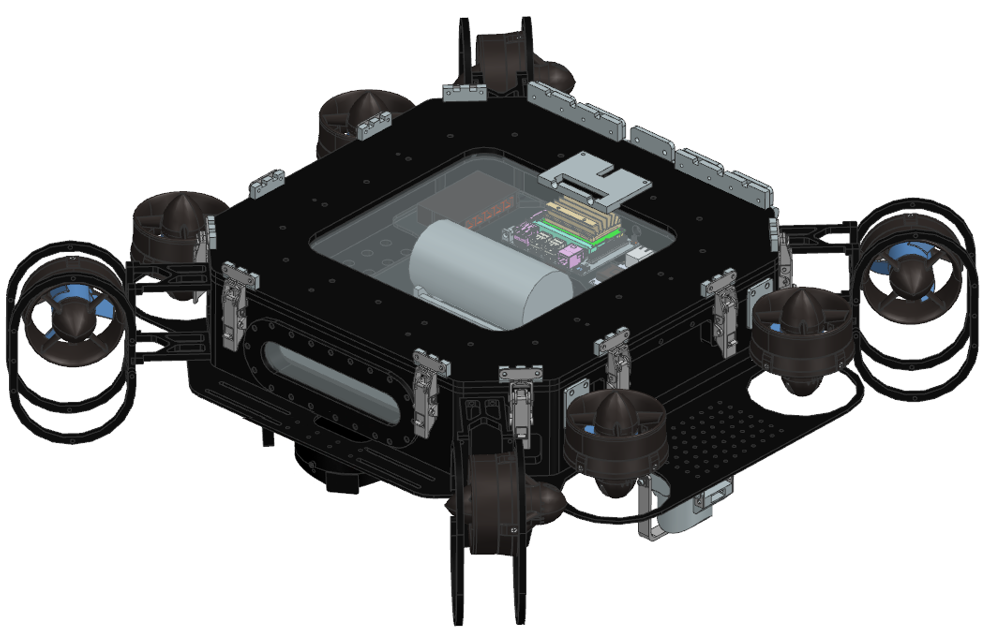
\includegraphics[scale=0.35]{images/FullSub2025-5.png}}
    \caption{CAD of our 2024-2025 AUV, Theseus.}
    \label{fig:sub4}
\end{figure}

\item \textit{Path:}
In order to reach the slalom and bins tasks, we intend to use the path-marker, which makes use of an additional camera on the bottom of the submarine.
Since we use classical computer vision algorithms for our relatively low-resolution bottom camera, this sub-system draws a reasonably low amount of computing power. Should this system fail, we can use a hard-coded “fallback” orientation, making the system sufficiently reliable to offset its associated complexity.

\item \textit{Navigate the Channel---Slalom:}
We also aim to achieve maximum points on the slalom task by identifying and properly navigating the slalom. To identify the red center slalom pole, we utilize the large horizontal field of view (110°) of our front-facing stereo camera along with a computer vision algorithm to detect the pipe based on its shape and color. We decided to use a classical computer vision algorithm rather than machine learning for this task since classical algorithms excel at detecting simple colors and shapes, and do not require the extensive data and training that machine learning does. This simplicity allows us to complete this task for maximum points without having to tune complex models.

\item \textit{Drop a BRUVS---Bins:} We intend to complete the bins task for the first time, maximizing points by dropping two markers into the side of the bin coordinated with the slalom and gate tasks. For this task we designed a dropper mechanism with simplicity in mind which resulted in consistent and reliable dropping of a single marker. As such, there is a dropper mechanism mounted on either side of Theseus to improve the symmetry for hydrodynamic forces and point-scoring potential. Similarly to the slalom task, we chose to use classical computer vision rather than machine learning to detect the bin due to its simple shape and color. To center on the bin, we alternate descending and re-centering on the bin, switching between the two based on the visual distance to the center of the bin in the image from the bottom camera. We do these movements separately rather than simultaneously to reduce the potential of roll/pitch movements causing the camera to lose sight of the bin. 

\item \textit{Return Home}: Should the vehicle complete some or all of the other tasks we set out to accomplish, we intend for the vehicle to return to the start to claim additional points. This may utilize the vehicles localization capabilities or be pre-programmed depending on the success of the other tasks.
\end{enumerate}



\section{Design Creativity}
\label{sec:design}


\subsection{Mechanical}
\label{ssec:mechanical}

\begin{figure}[h]
    \centerline{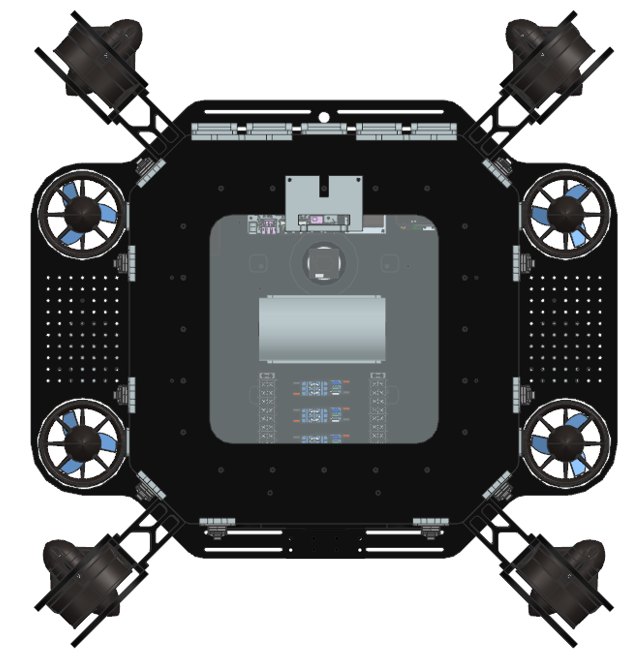
\includegraphics[scale=0.35]{images/FullSub2025Top.png}}
    \caption{CAD of top-view of Theseus.}
    \label{fig:sub3}
\end{figure}

\subsubsection{Hull}
\label{sssec:hull}
Our hull is machined from 6061 aluminum with half inch walls to allow for long term reusability. It is a component we recovered from our previous AUV reduce manufacturing costs, and its modularity characteristics enable easy modifications. It has three windows, two for a front camera and bottom camera and one that provides visibility to the electrical systems for quick troubleshooting. A double o-ring face seal was used at each port to create a redundant seal that ensures a reliable leak proof sub. A lid is mounted to the hull via hinges and secured in place using latches when the sub is underwater. This hinge and latch system makes accessing electronics a quick and simple process. The submarine also contains an eight-thruster configuration, allowing it to move in all six degrees of freedom.

Besides the hull, our AUV was completely refurbished and redesigned for strength and modularity. With additional components this year, including a grabber and a dropper mechanism, we had to modify the frame around our hull to allow for the mounting of these components while also keeping the vehicle light enough to be at least slightly positively buoyant. We machined and installed a new bottom plate with a plethora of holes and slots to allow us to shift components and ballast weights as we test for weight distribution purposes and prevent unnecessary redesigns. This bottom plate also served the purpose of protecting the sub’s vertical thrusters from impacts. 

In addition to redesigning the AUV’s bottom plate, we also machined new mounts for its angled thrusters. These mounts contained thruster shrouds to protect from wall collisions. These shrouds, as well as a new bottom plate, increased the weight of the sub. To account for this additional weight, we redesigned the lid of our hull, primarily reducing its thickness, and by extension, its weight. This redesign allowed us to discard a significant portion of buoyancy foam mounted to the top of the vehicle. 


\subsubsection{Grabber}
\label{sssec:grabber}
To collect and move samples, we implemented a claw mechanism (Fig \ref{fig:grabber}). Our design features four motor-actuated claws linked through a set of worm gears and axles, allowing for a more secure hold on the sample. When the motor spins in one direction, the worm gear spins, causing the claws to move farther apart until a wide enough gap between them opens for them to grab a sample. Meanwhile, clamping onto the sample is a simple matter of reversing the motors to close and secure the sample. The arms and supporting frame were SLA 3D printed due to their complicated geometries. They are stiff enough to pick things up and hold them, while still remaining weaker than the rest of the mechanism so that they break first in case of a collision, since they are much easier to make and less expensive to replace.

\begin{figure}
    \centerline{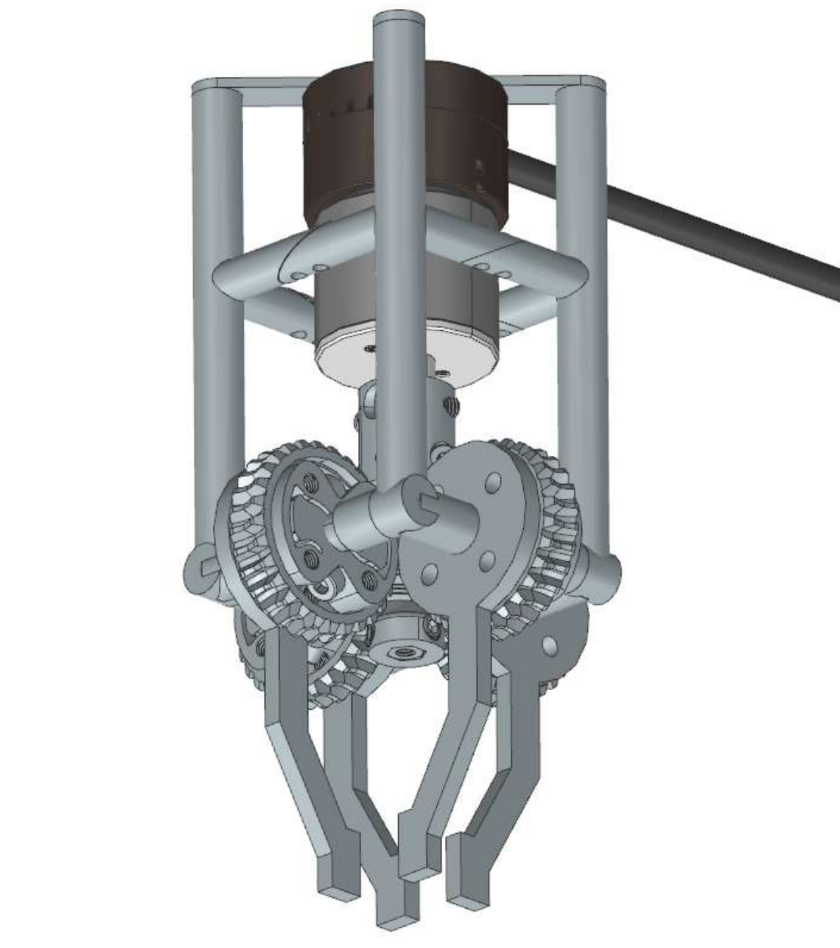
\includegraphics[scale=0.22]{images/grabber2025.png}}
    \caption{CAD of our grabber.}
    \label{fig:grabber}
\end{figure}

\subsubsection{Dropper}
\label{sssec:dropper}
This year, we also implemented a marker dropper subsystem (Fig \ref{fig:dropper}). Rather than employing one dropper containing two markers, we incorporated two identical droppers, with one marker in each to improve the reliability by eliminating the possibility that two markers would unintentionally be dropped simultaneously. Each dropper consists of a 3D printed tubular hopper in which the marker is stored. To hold the marker in place before an intended drop, a bent sheet metal arm covers the bottom opening of the tube. To release the marker, a servo connected to this arm is actuated, uncovering the bottom opening of the tube and allowing the marker to fall. 3D printing the marker dropper hoppers was a quick and easy way to produce the complex shapes incorporated into the design.

\begin{figure}
    \centerline{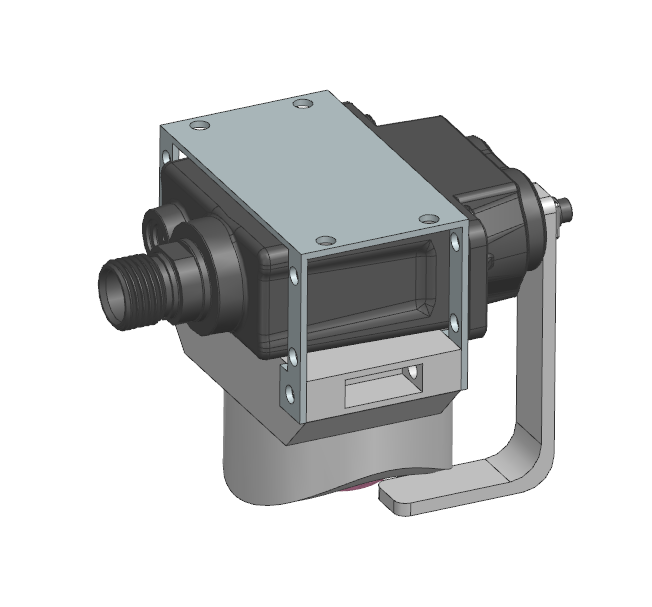
\includegraphics[scale=0.22]{images/dropperNew.png}}
    \caption{CAD of our dropper.}
    \label{fig:dropper}
\end{figure}

\subsection{Electrical}
\label{ssec:electrical}

\subsubsection{Newly Created Sub-Team}
\label{sssec:electrical_subteam}
This year, we saw an unprecedented growth in students interested in developing electronics crucial to our AUV. Thus, to more effectively lead and compartmentalize our team, we separated the electrical sub-team from the software team. To facilitate this transition, we invested time and energy in gently onboarding the new members (many of whom were freshmen) and familiarizing them with the submarine and the team.

\subsubsection{Fuses}
\label{sssec:fuses}
After experiencing an electrical fire while live testing the AUV, we decided to implement fuses on multiple components. Accordingly, we ran fuses to each of our motor control boards which we believe may be prone to electrical fires, as well as our Doppler Velocity Log (DVL) because of how expensive it would be to replace it. We used in-line fuses for a quick and reliable solution, with future plans to integrate current protection into our PCBs. 

\subsubsection{Hall Effect Sensors}
\label{sssec:hall_effects}
To control the behavior of the AUV while disconnected from its tether, we used two latching hall effect sensors. Magnets trigger these sensors to control the starting, stopping, and resetting of other sensors (in particular, the IMU) without needing a live connection. The ability to quickly control the state of our sensors externally improves the efficiency of our testing setup time. Once a state is activated, an indicator LED is lit for visual verification. 

This year, we designed a custom PCB and 3D printed mount for our hall effect system. Previously, the hall effect sensors faced frequent disconnections due to loose wires and was difficult to troubleshoot due to wire overcrowding. The hall effect PCB and mount remedied this issue by quartering the number of wires and organzing components to ease troubleshooting.

\subsubsection{Motor Control Board}
\label{sssec:motor_board}
We identified the motor control electrical subsystem as a top priority due to its critical functionality, frequency of maintenance, and large space overhead. Previously, each of our eight thrusters had 3 long wires routing across the bottom of the AUV's hull. These 24 wires would connect to eight electronic speed controllers (ESCs) and then output to eight PWM signals which are controlled by our new thruster mixing driver. In practice, this setup made the subsystem difficult to organize and maintain. For example, changing an ESC was intricate and prone to breaking other components. 

As a result, we chose to encapsulate all of these wires and components into a custom printed circuit board (Fig. \ref{fig:motor_pcb}). We now have two sets of Motor-ESC boards (one on each side of the robot), where each set takes input from 4 thrusters and outputs 4 PWM signals. The ESCs mount directly to the PCB with screw-block terminals, so we can easily unscrew and swap them out. The thruster motors and PWM output connect to the PCB using Molex connectors which provide strong connections and can be disconnected easily if needed. This makes swapping out ESCs easier when necessary and frees space inside the AUV for other components.

\begin{figure}[htbp]
    \centerline{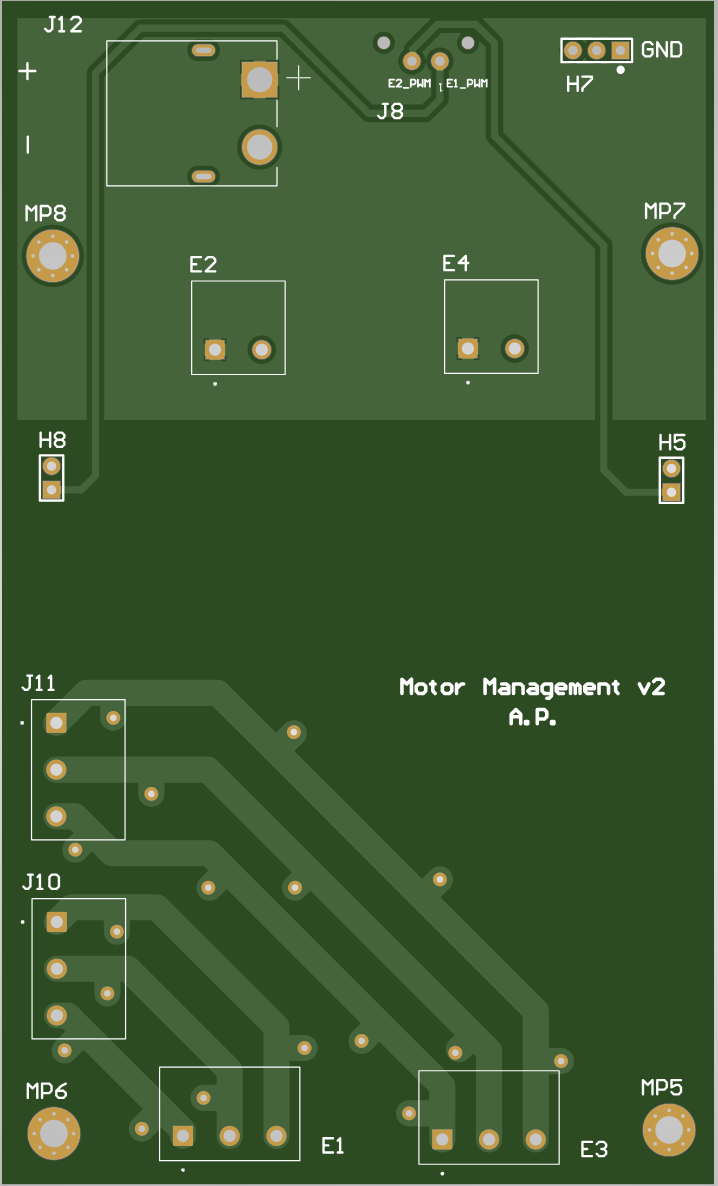
\includegraphics[scale=0.3]{images/motor_pcb.png}}
    \caption{Motor control board PCB design}
    \label{fig:motor_pcb}
\end{figure}

An important consideration was the current limit for this PCB. The first iteration of this board was operational but failed during prolonged water testing due to insufficient current rating and heat dissipation. The issue was that each ESC could theoretically draw up to 30A which meant the board’s traces had to support this requirement. Increasing the trace width to support 30A was not a good use of space, so we decided to increase the copper weight of each trace, essentially making them ``taller." Additionally, we used techniques like dissipating heat with thermal vias and large power and ground planes to fully allow our motor control board to work with multiple ESCs and motors for the second iteration of the board which is currently in use.

\subsubsection{Voltage Regulation}
\label{sssec:voltage_regulation}
We continue to use our custom power distribution PCB, which utilizes an off-the-shelf Pololu 5V 15A Step Down Regulator as our DC-DC converter to supply up to 75 W to most of our electrical system components. We utilize a separate OTS DC-DC converter to supply the Jetson Xavier NX with 13V.

\begin{figure}[htbp]
    \centerline{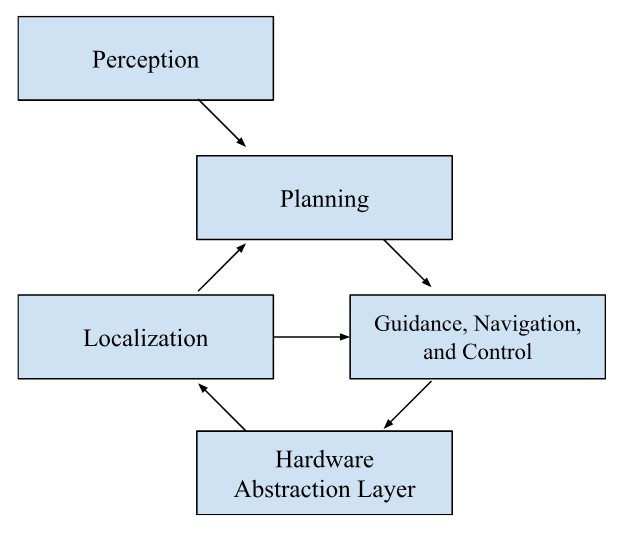
\includegraphics[scale=0.47]{images/ros_diagram.jpg}}
    \caption{High-level Software Architecture}
    \label{fig:ros}
\end{figure}
\subsection{Software}
\label{ssec:software}

Our software stack utilizes the Robot Operating System (ROS) to distribute our logic into distinct modules called nodes. These nodes are organized into packages based on their role in the AUV's operation. Fig. \ref{fig:ros} shows these packages, with arrows representing the general flow of information between packages. The majority of our code is written in Python, with the exception of some portions of the hardware abstraction layer, which is written in C. 

\subsubsection{Computing Architecture}
\label{sssec:comp_arch}
Our computing architecture features a distributed layout to enable high flexibility and faster iteration speed. Most of our computing is performed on our Jetson Xavier NX. This is the most powerful computer in the system, so it is responsible for running our computer vision, machine learning, high-level planning, localization, and control modules. Until last year, our motor control was handled by a Pixhawk PX4 flight controller using a Raspberry Pi 3B+ as an interface. To reduce technical complexity and weight, we replaced the Pixhawk PX4 and Raspberry Pi with our custom solutions that serve the same purpose: an Inertial Measurement Unit (IMU), a thruster control board and driver, and thruster mixing code. All of this now also runs on the Jetson Xavier NX. For interfacing with our low-power devices---namely our depth sensor, hall effect sensors, and indicator lights-–-we use an Arduino, which the Jetson communicates with via \verb|rosserial|.

\subsubsection{Flight Controller}
\label{sssec:flight_controller}
To replace the Pixhawk flight controller, we developed an in-house thruster mixing system and thruster control board driver. Our system was initially designed referencing Tartan AUV's thruster mixing and thruster control code.

The code uses the positions and orientations of the thrusters to construct a non-square matrix mapping the input powers for the eight motors to the vehicle wrench (force/torque in all six degrees of freedom). It then takes the pseudoinverse of this matrix to map desired wrench to motor powers. However, this mapping may request motor powers which exceed the maximum force output of the motor, or may request a motor configuration which draws excessive current, possibly degrading the electrical system of the vehicle. To combat this, the controller dynamically and uniformly scales down the requested input wrench until the computed motor powers fall within predefined power and current limits. The controller then uses a model to determine the input signal to be sent to each motor to produce the desired force, which is a nonlinear function. The relationship between motor input signal, motor output power, and motor current draw (all with respect to system voltage) was calculated by fitting cubic polynomials in the thruster's forward and reverse directions using data provided by the supplier, BlueRobotics. The polynomial relating PWM motor input and current is shown in Fig. \ref{fig:motor_fits}.

\begin{figure}[htbp]
    \centerline{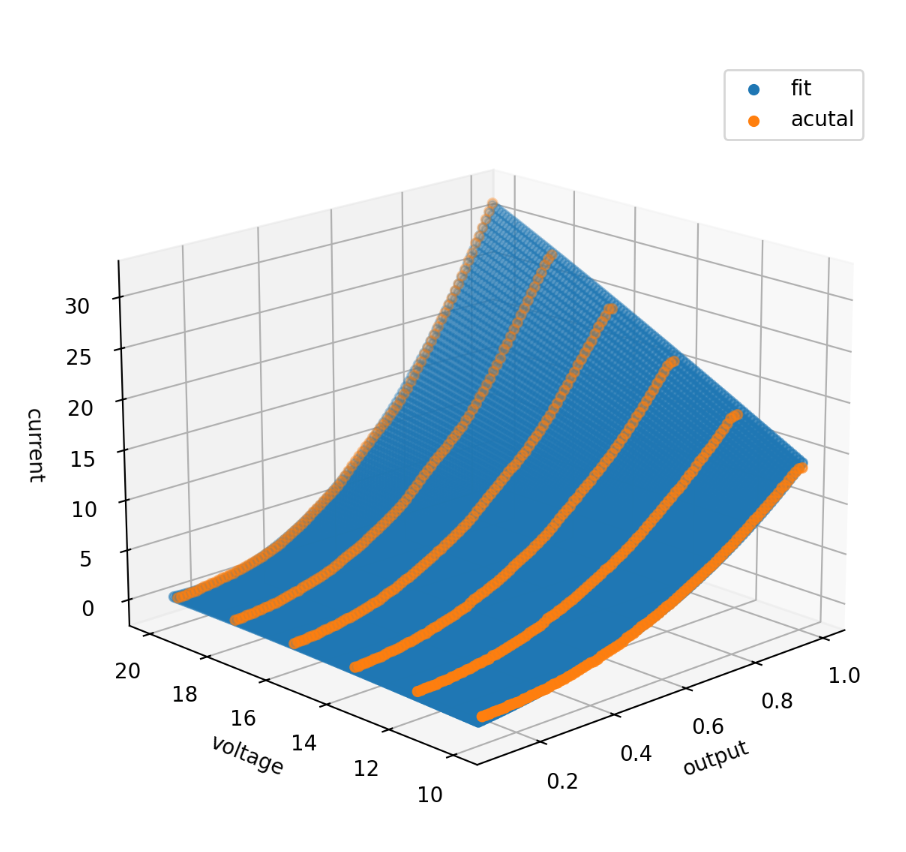
\includegraphics[scale=0.32]{images/motor_fits.png}}
    \caption{Computed motor fit curve relating input voltage, thruster mixing output (i.e., PWM motor input), and current draw.}
    \label{fig:motor_fits}
\end{figure}

\subsubsection{Orientation Sensing}
\label{sssec:orientation_sensing}
To measure our orientation, we use the InertialSense IK-1-IMX-5 IMU. This IMU was chosen for its high measurement frequency (1 KHz), low rate gyroscopic drift (claimed $0.16^{\circ}/\sqrt{hr}$), and built in Altitude, Heading, and Reference System (AHRS) which fuses measurements from the gyroscope, accelerometer, pressure, and magnetometer sensors into a single accurate orientation estimate. We use the IMU to measure linear acceleration and angular velocity along the x, y, and z axes. We also use the AHRS to provide orientation information to our planning and control algorithms.

\subsubsection{Computer Vision}
\label{sssec:cv}
In order to detect the pathmarker, slalom, and bins, we utilize classical computer vision (CV) techniques with the OpenCV library. The target objects are single-colored with few features, making them highly noticeable with HSV thresholding. The HSV (Hue, Saturation, Value) color model simplifies the process of detecting these objects, as it aligns closely with human perception of color and allows for intuitive color-based segmentation \cite{b2}. Additionally, CV techniques are computationally cheaper compared to ML models, making them more suitable for real-time applications.

Our HSV filter pipeline involves several steps to enhance and process the underwater images to detect, e.g., the path marker, slalom, and bins. First, we adjust the white balance---shifting and scaling the color channels---of the image to counteract underwater distortion and make objects more distinguishable. Next, we perform histogram equalization on the RGB channels of the image to enhance contrast, ensuring that object details stand out more prominently (Fig. \ref{fig:enhanced_compare}). The enhanced image is then converted from the RGB color space to the HSV color space. To reduce noise and smooth the image, we apply median and Gaussian filters. Next, we apply color thresholding to the HSV image to create a binary mask that isolates the object’s colors, which highlights the object against the background. The binary mask is further refined using morphological operations such as erosion and dilation to mitigate noise and fill gaps.


\begin{figure}[htbp]
    \centerline{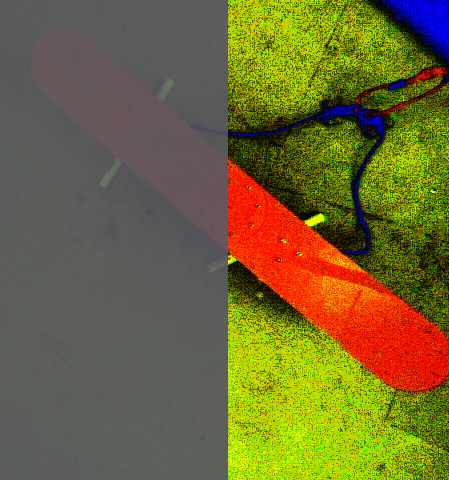
\includegraphics[scale=0.32]{images/pathmarker_compare.png}}
    \caption{Example of a pathmarker image before (left) and after (right) image enhancement.}
    \label{fig:enhanced_compare}
\end{figure}


Using the binary mask, we detect contours in the image, representing object boundaries. We analyze these contours by their size and features uniqueness to identify the desired objects. If a valid contour is found, we then process them based on the specific tasks: either path marker, buoy, or bin. For the path marker, we use the minimum area rectangle method (bounding box) to approximate the path marker's boundary. We then identify the corners of this rectangle and calculate the center points of the edges. The centers of the edges and the center of the rectangle are calculated, and we use these points to determine the yaw angle of the path marker relative to the camera's heading. By drawing lines between the corners and calculating the angles, we can determine the orientation of the path marker. This provided a significant improvement over our previous pathmarker detection algorithms, which naively searched for lines without considering the shape of the object. For bin detection, the process is analogous to path marker detection; Fig. \ref{fig:bin_features} shows an example of detecting the key features on the object. See Appendix A for full examples of this pipeline operating on each object type.

\begin{figure}[htbp]
    \centerline{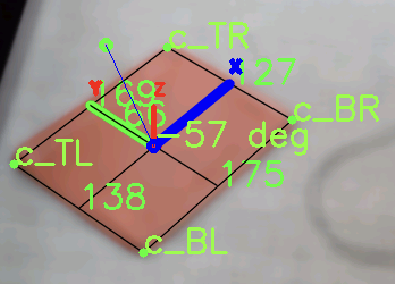
\includegraphics[scale=0.55]{images/bin_features.png}}
    \caption{Example of detecting key features on a bin-shaped object.}
    \label{fig:bin_features}
\end{figure}

One notable challenge we faced was the effects of our camera's automatic white-balance adjustments, which can introduce variability in the color representation of objects and thus affect the accuracy of HSV filtering under varying lighting conditions. To mitigate this issue, we used manual white-balance settings to maintain consistent color representation and enhance our CV pipeline's reliability. However, we were only able to disable the automatic white-balance setting on our downward-facing camera. Our forward-facing camera also encountered an issue in which the brightest white-balance setting introduced significant artifacts to the video stream. This issue was only encountered in the bright outdoor competition setting, so we employed the simple solution of blocking part of the image with tape to prevent the camera from ever switching to its brightest white-balance setting.

\subsubsection{Machine Learning}
\label{sssec:ml_flow}
To detect the images on the gate, we continue to use the machine learning pipeline that we developed in 2023. We use the YOLOv5 neural network \cite{b3} for object detection, which we fine-tuned to detect gate images. Our model runs within the PyTorch framework, an open source machine learning framework that is an industry standard for this type of work \cite{b4}. 

\subsubsection{Task Planner}
\label{sssec:task_planner}
The task planner is the code for coordinating system components to complete competition tasks. This year we introduced several new features to our task planning infrastructure to increase the iteration speed, catch additional issues during development, and more efficiently utilize our limited in-water testing time.

Our task planner follows a state machine framework, where the AUV is in one state at a time. Each state defines the logic commanding the motors given the current sensor inputs.

Our state machine defines the order of states and the conditions to transition from one state to another. We use several transition maps for various behavior routines, such as the standard map for complete competition runs, the bin map for testing approaching and completing the bin task, etc. Appendix B includes an generated diagram of our current competition state machine. We can use different maps at testing time to isolate the relevant behaviors.

Because our state machine infrastructure is written in Python, in previous years, issues regarding incorrect variable names and object types were not encountered until we were running the vehicle in the water. Such issues take up valuable time that could be spent gathering data and validating our vehicle. These issues can be mitigated with static analysis tools such as \verb|mypy|, a Python linter and type checker.

In the past few years, we have been significantly improving our state machine framework to catch errors before water-test time. This year, we reached the point where all of our planning code can be checked with \verb|mypy|. We now enforce this by requiring all code changes to our development branch pass the \verb|mypy| type checker using GitHub Actions. The additional type safety also helps our development environment to provide much more relevant auto-complete suggestions, increasing developer productivity. 

The state-transition-map system initially had a limitation: parameters defined on states (such as target depth or timeout period) could only be defined once among all transition maps, so switching between the competition pool and the testing pool (which may have different depths) required updating the code to change the target depth. This year, we added a parameter-overriding feature to override parameters for each transition map, allowing us to switch between testing regimes much faster. We also added the ability to start running the state machine from any state, rather than just the predefined start state, which helps to test the system faster.

\section{Testing and Experimental Results}
\label{sec:testing}

\subsection{Teleoperation Framework}
\label{ssec:teleop}
A key takeaway from competing in-person has been the need for an efficient water testing infrastructure. Due to the interdependence of our subsystems, it is challenging to test individual components of our system while the AUV is operating autonomously; it is often difficult to diagnose the source of errors when the entire system is running.

Last year, we developed a robust teleoperation (teleop) framework that allows a human driver to manually control various aspects of the AUV while other subsystems run autonomously, enabling us to execute unit tests and debug components in isolation. By writing our own teleop framework, we are not limited to any specific hardware or software such as ArduSub and are able to provide tighter integrations with our other systems. We can use the controller to directly activate and deactivate our state machine, alternate between controlling certain axes of control directly or indirectly via controlling target setpoints, and disable the motors immediately at the lowest level of control when the emergency-stop button is activated. This year, we continued to use this teleop framework and found that it greatly simplified testing and iteration.

\subsection{In-Water Testing}
\label{ssec:in_water_testing}
From past competitions we have learned that in-water testing is invaluable and allows for both the software and hardware teams to validate their designs. It is also a great opportunity to train new members and boost morale. For these reasons, our team has attempted to utilize our university's resources to perform as many water tests as possible.

This year, we performed our testing at the U-M Marine Hydrodynamics Laboratory (MHL) towing tank. This tank is large enough for us to calibrate sensors and motors, evaluate our control and localization algorithms, and test our state machine's interactions with game elements.

Before each in-water testing session, we prioritized which components we intended to test. Then after each session, we reviewed what we tested and what the results were, as well as any other issues/future improvements we found or thought of. 

At a training session late this past fall, we encountered an issue which damaged multiple components and required a full tear-down/rebuild of our vehicle's electrical system (see \ref{sssec:fuses}). We used this opportunity to train many new electrical team members and make significant changes to our electrical system. However, this also delayed when we could return to testing our new system components to later in the year. Many of our later test sessions were used to validate the new changes and collect data for offline testing and improvements.

\subsection{Off-Board Testing}
\label{ssec:off_board_testing}
To prevent us from wasting in-water testing time on simple software errors, we developed a container image that emulates our main computer to use with virtualization software like Docker and Podman. This allows any team member to write, execute, and test our software off the AUV on their laptop. In general, we test the logic of our software within the container and reserve in-water testing for collecting data to improve our vision system or testing the physical results of our algorithms once they had been tested in simulation. 

To visualize the state of our vehicle, we created visualizations using RQt, a ROS dashboard library. We leveraged RQt to graph data and dynamically tune control parameters, allowing for easy incremental testing.

\section*{Acknowledgments}

The Michigan Robotic Submarine team would like to thank our 2025 sponsors for their monetary support: Ford Motor Company, University of Michigan Central Student Government, University of Michigan Engineering Student Government, the University of Michigan College of Engineering along with the departments: Robotics, Computer Science and Engineering, Electrical and Computer Engineering, and Mechanical Engineering. We'd also like to thank the individuals who donated to our team during the University of Michigan's Giving Blue Day fundraiser.

In addition, we would like to thank our advisor Dr. Katie Skinner for continuously supporting our team by advising us and overseeing the Multidisciplinary Design Program which allows members to earn class credit for their contributions to our team.

We are greatly appreciative of the Marine Hydrodynamics Lab staff, especially Jason Bundoff and Nicole Cheesman, for graciously providing the team with an in-water testing location. 

We also would like to thank the Wilson Student Team Project Center facilities and Ford Motor Company Robotics Building staff, especially Alyssa Emigh and Chris Gordan, for hosting our team workspace, providing tools and resources, and supporting our endeavors. 

We are also thankful of Mariah Moss and Katelyn Poore from the Office of Student Affairs at the University of Michigan College of Engineering for their guidance in developing our team and assistance purchasing the materials that make our work possible. 

Lastly, we would like to thank the RoboNation team for organizing the RoboSub competition. We are also thankful for image data provided through the RoboNation data sharing program.

\begin{thebibliography}{00}
\bibitem{b2} N. Fragoulis and D. Kastaniotis, “Why Embedded Software
Development Still Matters: Optimizing a Computer Vision Application
on the ARM Cortex A8.” 2013, publisher: Irida Labs. [Online].
Available: http://rgdoi.net/10.13140/2.1.2670.6240
\bibitem{b3} G. Jocher, ``ultralytics/yolov5: v6.1 - TensorRT, TensorFlow Edge TPU and OpenVINO Export and Inference”. Zenodo, Feb. 22, 2022. doi: 10.5281/zenodo.6222936.
\bibitem{b4}{P. Adam et al., ``PyTorch: An Imperative Style, High-Performance Deep Learning Library", in Advances in Neural Information Processing Systems 32, Curran Associates, Inc., 2019, pp. 8024–8035.}
\bibitem{b5} Inspiration Robotics, ``RoboSub-Simulation". Github.com. https://github.com/InspirationRobotics/RoboSub-Simulation (accessed June 11, 2022)

\end{thebibliography}

\clearpage
\appendices

\raggedbottom

\pagebreak
\section{Computer Vision Pipeline Results}

\vspace{0.5cm}
\includegraphics[scale=0.42]{images/cv_pipeline.drawio.png}
\newpage
\clearpage


\section{State Machine Diagram}
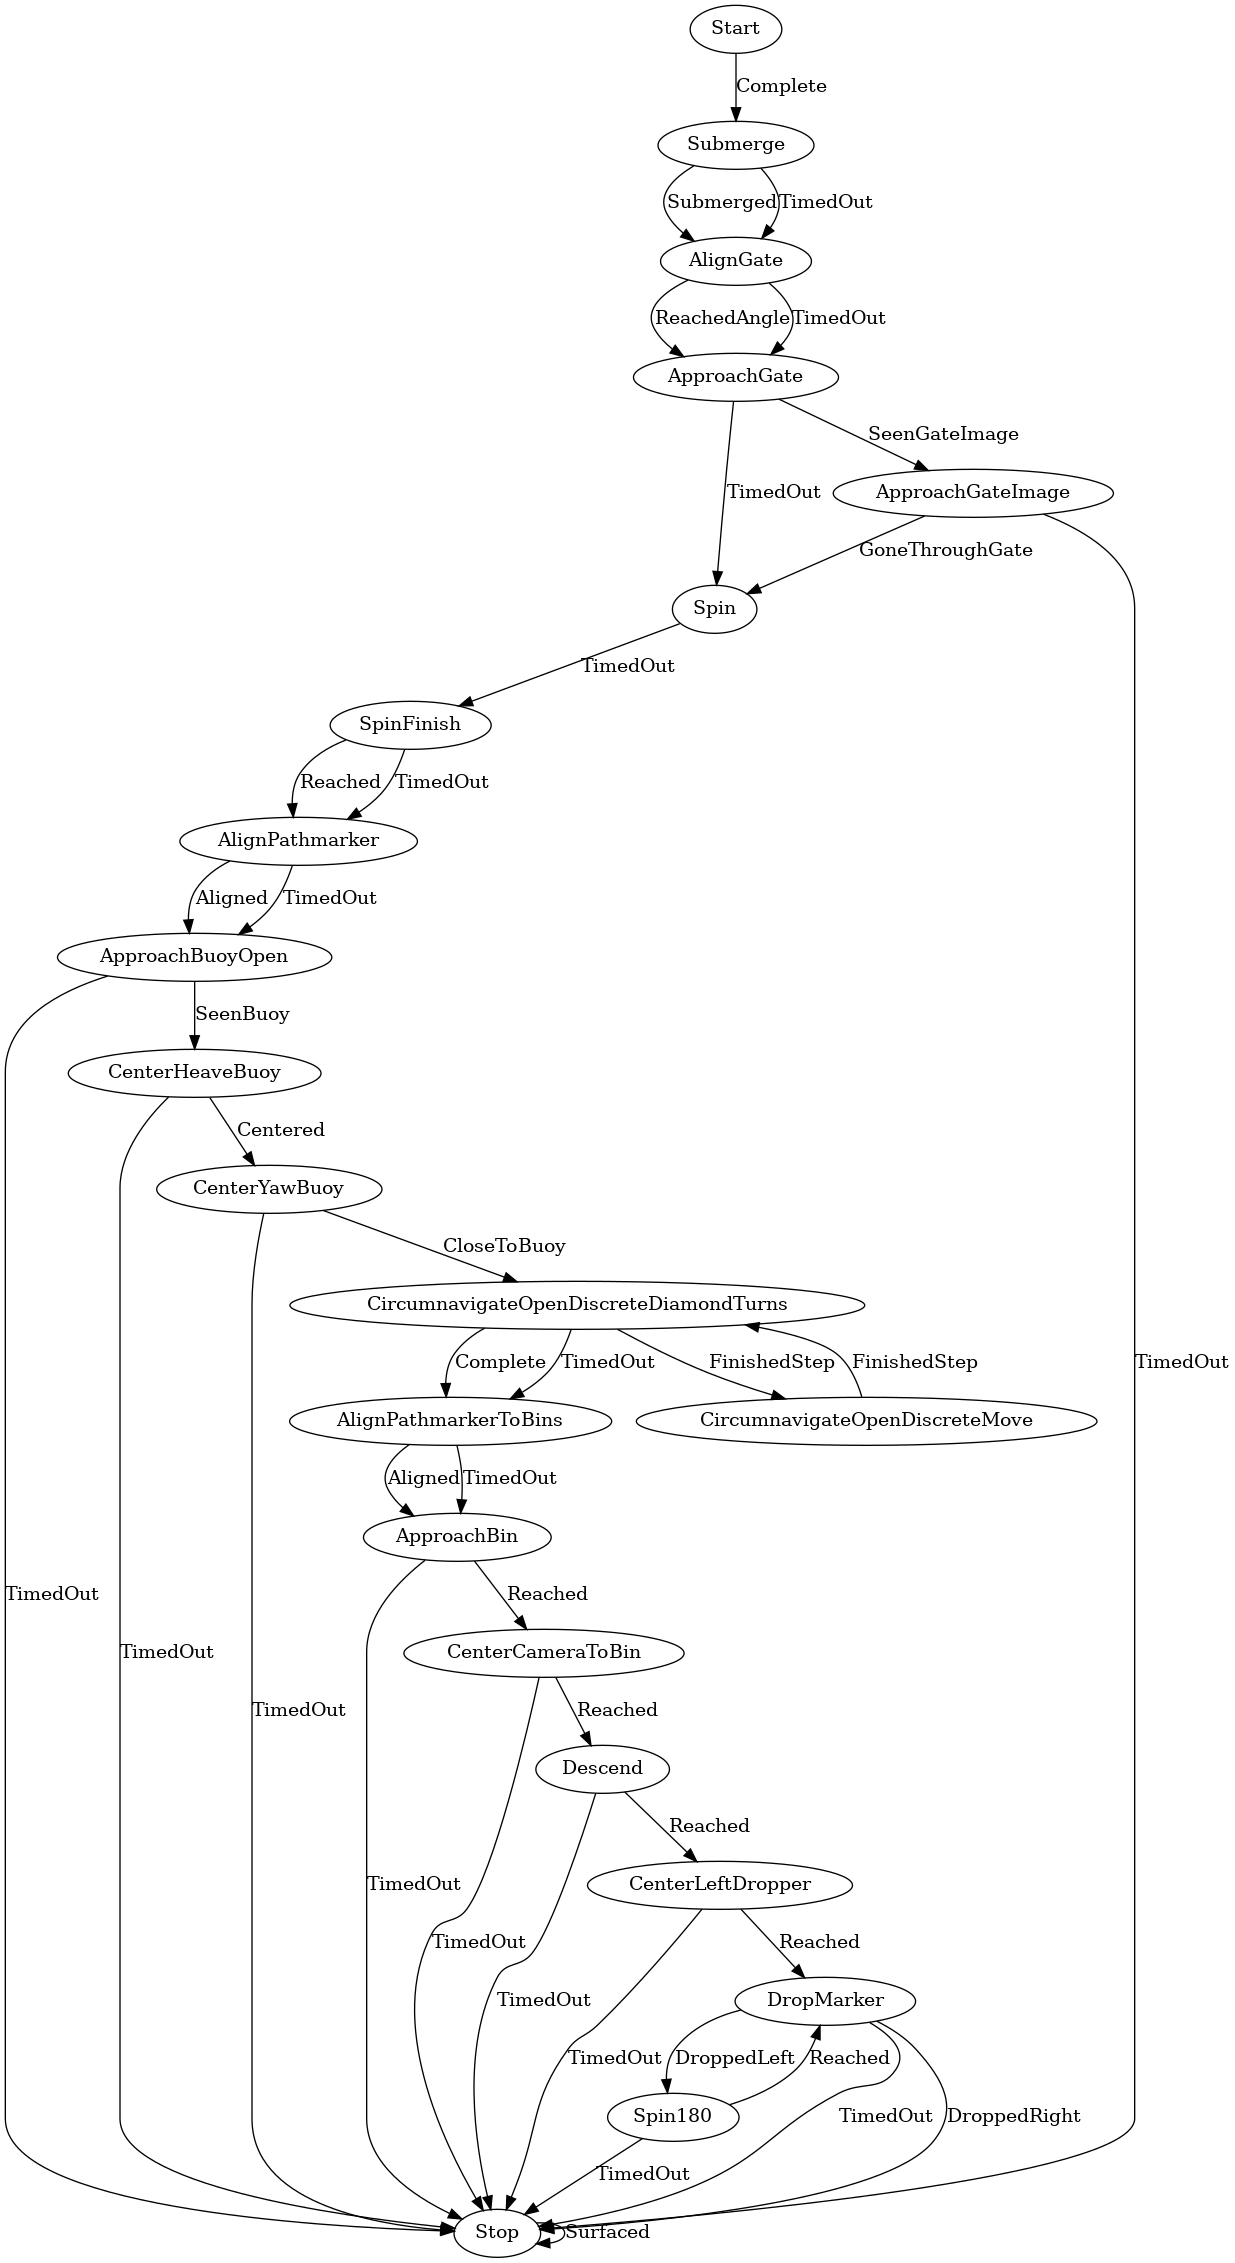
\includegraphics[scale=0.27]{images/machine2.png}
\newpage

\clearpage
\section{Component Specifications}

\begin{table}[htbp]
\begin{tabularx}{\textwidth}{|L|L|L|L|L|L|}
    \hline
        Component & Vendor & Model/Type & Specs & Cost (if new) & Year of Purchase \\ \hline
        ASV Hull Form/Platform  & American Tooling \& Prototype & Custom & 6061 Aluminum & \$3250.00 & 2022 \\ \hline
        Waterproof Connectors & Blue Robotics & WetLink Penetrators & WLP-M10-6.5MM-HC & \$120.00 & 2024 \\ \hline
        Propulsion  & Blue Robotics & T200 w/ Propellor & 7-20V & \$1,074.00  & 2020\\ \hline
        Power System & N/A & Custom & N/A & N/A & N/A \\ \hline
        Motor Controls  & Blue Robotics & Basic ESC & 7-26V & \$172.00  & 2023 \\ \hline
        CPU & Nvidia & Jetson Xavier NX & 6-core Nvidia Carmel ARM v8.2 @ 1.9 GHz, 16 Gb RAM & \$400.00  & 2022 \\ \hline
        Thruster Control Board  & Pololu & Mini Maestro 12 & 12-Channel USB Servo Controller & \$37.95  & 2024 \\ \hline
        Inertial Measurement Unit (IMU)  & Inertial Sense & IK-1-IMX-5 & Accel/Gyro: 10-DOF sensor & \$350 & 2025 \\ \hline
        Doppler Velocity Log (DVL) & Cerulean Sonar & Tracker 650 & Uses 3 velocity sensors. Maximum depth rating: 300m & \$2,990 & 2024 \\ \hline
        Camera(s) & Stereolabs, Blue Robotics & ZED2, Low-light HD USB Camera & stereo vision, pathmarker detection & \$449.00, \$99.00  & 2020, 2021 \\ \hline
        Localization and Mapping  & N/A & Custom & N/A & N/A & N/A \\ \hline
        Vision  & N/A & YOLOv5, PyTorch, OpenCV & train convolutional neural network and perform classical computer vision & N/A & 2023 \\ \hline
        Autonomy  & N/A & Custom & N/A & N/A & N/A \\ \hline
        Open source software & N/A & Andy Ze ROS PID & PID Control & N/A & N/A \\ \hline
    \end{tabularx}
\label{tab1e}
\end{table}



\end{document}
